\documentclass[pdflatex,sn-mathphys-num]{sn-jnl}

\usepackage{graphicx}
\usepackage{booktabs}
\usepackage{amsmath,amssymb,amsfonts}
\usepackage{amsthm}
\usepackage{xcolor}
\usepackage{array}
\usepackage{tabularx}
\usepackage{microtype}
\setlength{\emergencystretch}{2em}

\raggedbottom
% Auto-generated by scripts/run_benchmark.py from results/tables/*.csv — DO NOT EDIT BY HAND
\newcommand{\TotalClips}{2,353}
\newcommand{\TotalPos}{708}
\newcommand{\TotalNeg}{1,645}
\newcommand{\TotalPosPct}{30.1\%}
\newcommand{\TotalScenes}{175}
\newcommand{\DupTotal}{255}
\newcommand{\DupMNNIT}{15}
\newcommand{\DupShop}{218}
\newcommand{\DupUCF}{22}
\newcommand{\ParentUCF}{28}
\newcommand{\PooledAUROCID}{0.725}
\newcommand{\MacroAUROCID}{0.500}
\newcommand{\PooledAUROCBias}{+0.225}
\newcommand{\PooledAUPRCID}{0.472}
\newcommand{\MacroAUPRCID}{0.291}
\newcommand{\PooledAUPRCBias}{+0.181}
\newcommand{\DCSASSRand}{0.907}
\newcommand{\DCSASSNom}{0.566}
\newcommand{\DCSASSStr}{0.566}
\newcommand{\DCSASSDrop}{0.341}
\newcommand{\MNNITRand}{0.971}
\newcommand{\MNNITNom}{0.954}
\newcommand{\MNNITStr}{0.928}
\newcommand{\MNNITDrop}{0.043}
\newcommand{\ShopRand}{1.000}
\newcommand{\ShopStr}{0.877}
\newcommand{\ShopDrop}{0.122}
\newcommand{\BestZSMacro}{0.690}
\newcommand{\BestZSLo}{0.631}
\newcommand{\BestZSHi}{0.748}
\newcommand{\BestTRMacro}{0.670}
\newcommand{\BestTRLo}{0.609}
\newcommand{\BestTRHi}{0.722}
\newcommand{\LFourteenTRMacro}{0.512}
\newcommand{\LFourteenTRLo}{0.435}
\newcommand{\LFourteenTRHi}{0.576}
\newcommand{\TopPairDiff}{+0.020}
\newcommand{\TopPairLo}{-0.051}
\newcommand{\TopPairHi}{+0.085}

% Auto-generated tables from results/tables/*.csv — DO NOT EDIT BY HAND

\newcommand{\TableCorpora}{%
\begin{table}[ht!]
\caption{Summary of the four deduplicated benchmark corpora (\TotalClips{} clips total, \TotalPos{} positives = \TotalPosPct{}) after removing \DupTotal{} SHA-256 byte duplicates (\DupMNNIT{} in MNNIT-S3, \DupShop{} in Shop-Dataset, \DupUCF{} in UCF-Crime) and \ParentUCF{} cross-corpus parent videos.}\label{tab:corpora}
\scriptsize
\setlength{\tabcolsep}{3pt}
\begin{tabular*}{\textwidth}{@{\extracolsep{\fill}}lrrrrrrl@{}}
\toprule
Dataset & Clips & Pos.\ (\%) & Neg. & Nom.\ grp. & Scenes & Scene size & Scene definition \\
\midrule
DCSASS~\cite{dcsass} & 896 & 155 (17.3\%) & 741 & 28 & 28 & 32--32 & Incident source folder \\
MNNIT-S3~\cite{mnnitmendeley,mnnitkaggle} & 574 & 207 (36.1\%) & 367 & 366 & 64 & 2--32 & Spherical $k$-means (CLIP-B/16) \\
Shop-Dataset~\cite{shopkaggle} & 581 & 324 (55.8\%) & 257 & --$^{\mathrm{a}}$ & 15 & 12--70 & Spherical $k$-means (CLIP-B/16) \\
UCF-Crime~\cite{sultani2018} & 302 & 22 (7.3\%) & 280 & 302 & 68 & 1--15 & Spherical $k$-means (CLIP-B/16) \\
\midrule
\textbf{Total} & \textbf{2,353} & \textbf{708 (30.1\%)} & \textbf{1,645} & -- & \textbf{175} & \textbf{1--70} & -- \\
\bottomrule
\end{tabular*}
\footnotetext{$^{\mathrm{a}}$Nominal folders in Shop-Dataset are segregated by class label (\texttt{shop lifters} vs.\ \texttt{non shop lifters}), so holding out a nominal folder leaves a single class in the test fold and AUROC is undefined.}
\end{table}
}

\newcommand{\TablePooledAudit}{%
\begin{table}[ht!]
\caption{Audit of pooled vs.\ unweighted macro evaluation using a trivial Dataset-Identity-Only predictor (assigning every clip the constant positive base rate of its source corpus without inspecting visual features).}\label{tab:pooled_audit}
\scriptsize
\setlength{\tabcolsep}{3.5pt}
\begin{tabular*}{\textwidth}{@{\extracolsep{\fill}}lccccccc@{}}
\toprule
Predictor & DCSASS & MNNIT-S3 & Shop-Dataset & UCF-Crime & Macro & Pooled & Pooled Bias ($\Delta$) \\
\midrule
Dataset-Identity-Only (AUROC) & 0.500 & 0.500 & 0.500 & 0.500 & \textbf{0.500} & \textbf{0.725} & $+0.225$ \\
Dataset-Identity-Only (AUPRC) & 0.173 & 0.361 & 0.558 & 0.073 & \textbf{0.291} & \textbf{0.472} & $+0.181$ \\
\bottomrule
\end{tabular*}
\end{table}
}

\newcommand{\TableSplitAudit}{%
\begin{table}[ht!]
\caption{In-domain 5-fold cross-validation AUROC (mean $\pm$ SD across 2 seeds) of the trained MIL head on frozen CLIP ViT-B/16 features under three split rules. Drops are computed from unrounded AUROC values.}\label{tab:split_audit}
\footnotesize
\setlength{\tabcolsep}{4pt}
\begin{tabular*}{\textwidth}{@{\extracolsep{\fill}}lcccc@{}}
\toprule
Dataset & Random clips & Nominal groups & Strict scenes & Drop ($\text{Random} \to \text{Strict}$) \\
\midrule
DCSASS & $0.907 \pm 0.003$ & $0.566 \pm 0.041$ & $0.566 \pm 0.041$ & $-0.341$ \\
MNNIT-S3 & $0.971 \pm 0.000$ & $0.954 \pm 0.001$ & $0.928 \pm 0.001$ & $-0.043$ \\
Shop-Dataset & $1.000 \pm 0.000$ & -- & $0.877 \pm 0.005$ & $-0.122$ \\
\bottomrule
\end{tabular*}
\end{table}
}

\newcommand{\TableLODO}{%
\begin{table}[ht!]
\caption{Leave-one-dataset-out (LODO) AUROC per held-out corpus, unweighted macro AUROC (with 95\% scene-cluster bootstrap CI over 500 replicates), macro AUPRC, and macro false alarm rate at 80\% recall ($\text{FAR@80\%R}$).}\label{tab:lodo}
\scriptsize
\setlength{\tabcolsep}{2.5pt}
\begin{tabular*}{\textwidth}{@{\extracolsep{\fill}}llcccccccc@{}}
\toprule
Backbone & Method & DCSASS & MNNIT-S3 & Shop & UCF & Macro AUROC & 95\% CI & AUPRC & FAR@80 \\
\midrule
\multicolumn{10}{@{}l}{\textit{Training-free zero-shot text-prompt baselines}} \\
CLIP-B/16 & \texttt{zs\_single\_max} & 0.575 & 0.684 & \textbf{0.645} & 0.837 & 0.685 & (0.602--0.754) & 0.456 & 0.534 \\
CLIP-B/16 & \texttt{zs\_ens8\_mean} & 0.528 & \textbf{0.810} & 0.539 & \textbf{0.884} & \textbf{0.690} & \textbf{(0.631--0.748)} & \textbf{0.479} & \textbf{0.512} \\
CLIP-B/16 & \texttt{zs\_ens8\_max} & 0.582 & 0.806 & 0.577 & 0.790 & 0.689 & (0.613--0.765) & 0.468 & 0.521 \\
SigLIP-B/16 & \texttt{zs\_single\_max} & 0.554 & 0.691 & 0.557 & 0.843 & 0.661 & (0.605--0.709) & 0.438 & 0.562 \\
SigLIP-B/16 & \texttt{zs\_ens8\_mean} & 0.527 & 0.749 & 0.439 & 0.862 & 0.644 & (0.594--0.695) & 0.429 & 0.584 \\
SigLIP-B/16 & \texttt{zs\_ens8\_max} & 0.503 & 0.792 & 0.424 & 0.878 & 0.649 & (0.600--0.700) & 0.435 & 0.575 \\
CLIP-L/14 & \texttt{zs\_single\_max} & \textbf{0.611} & 0.650 & 0.582 & 0.766 & 0.652 & (0.589--0.710) & 0.431 & 0.579 \\
CLIP-L/14 & \texttt{zs\_ens8\_mean} & 0.486 & 0.802 & 0.495 & 0.837 & 0.655 & (0.610--0.704) & 0.442 & 0.568 \\
CLIP-L/14 & \texttt{zs\_ens8\_max} & 0.521 & 0.801 & 0.462 & 0.856 & 0.660 & (0.599--0.718) & 0.446 & 0.559 \\
\midrule
\multicolumn{10}{@{}l}{\textit{Supervised MIL heads trained on the remaining three corpora (3-seed mean)}} \\
CLIP-B/16 & \texttt{trained\_head} & 0.595 & 0.723 & 0.626 & 0.737 & 0.670 & (0.609--0.722) & 0.448 & 0.546 \\
CLIP-L/14 & \texttt{trained\_head} & 0.505 & 0.798 & 0.328 & 0.416 & 0.512 & (0.435--0.576) & 0.334 & 0.732 \\
\bottomrule
\end{tabular*}
\end{table}
}

\newcommand{\TableAblations}{%
\begin{table}[ht!]
\caption{LODO ablation of unsupervised scene-mean centering ($\ge 8$ clips per scene) and Group-DRO reweighting on the supervised Top-3 MIL head (Part A), and sensitivity of LODO/CV AUROC to preprocessing constants (Part B: canonical OpenAI CLIP green-channel mean $0.4578275$ and duration $>20$\,s seek vs.\ perturbed $0.4728275$ and size $>15$\,MB seek).}\label{tab:ablations}
\scriptsize
\setlength{\tabcolsep}{2.5pt}
\begin{tabular*}{\textwidth}{@{\extracolsep{\fill}}llcccccc@{}}
\toprule
\multicolumn{8}{@{}l}{\textbf{Part A: Scene-mean centering and Group-DRO regularizers (LODO AUROC)}} \\
Backbone & Variant & DCSASS & MNNIT-S3 & Shop & UCF & Macro AUROC & 95\% CI \\
\midrule
CLIP-B/16 & \texttt{base} & 0.595 & 0.723 & 0.626 & 0.737 & 0.670 & (0.609--0.722) \\
CLIP-B/16 & \texttt{center} & 0.588 & 0.715 & 0.618 & 0.729 & 0.663 & (0.601--0.718) \\
CLIP-B/16 & \texttt{dro} & 0.599 & 0.726 & 0.621 & 0.742 & 0.672 & (0.611--0.726) \\
CLIP-B/16 & \texttt{center+dro} & 0.591 & 0.719 & 0.614 & 0.734 & 0.665 & (0.603--0.720) \\
CLIP-L/14 & \texttt{base} & 0.505 & 0.798 & 0.328 & 0.416 & 0.512 & (0.435--0.576) \\
CLIP-L/14 & \texttt{center} & 0.518 & 0.784 & 0.392 & 0.468 & 0.541 & (0.468--0.605) \\
CLIP-L/14 & \texttt{dro} & 0.512 & 0.801 & 0.341 & 0.432 & 0.522 & (0.446--0.585) \\
CLIP-L/14 & \texttt{center+dro} & 0.524 & 0.789 & 0.405 & 0.479 & 0.549 & (0.476--0.612) \\
\midrule
\multicolumn{8}{@{}l}{\textbf{Part B: Preprocessing sensitivity check (Canonical vs.\ Perturbed constants)}} \\
\multicolumn{4}{@{}l}{Evaluation metric / model} & \multicolumn{2}{c}{Canonical ($0.4578$, $>20$\,s)} & Perturbed ($0.4728$, $>15$\,MB) & Shift ($\Delta$) \\
\midrule
\multicolumn{4}{@{}l}{CLIP-B/16 \texttt{zs\_ens8\_mean} (LODO Macro AUROC)} & \multicolumn{2}{c}{0.690} & 0.692 & $+0.002$ \\
\multicolumn{4}{@{}l}{CLIP-B/16 \texttt{zs\_ens8\_max} (LODO Macro AUROC)} & \multicolumn{2}{c}{0.689} & 0.683 & $-0.006$ \\
\multicolumn{4}{@{}l}{CLIP-B/16 \texttt{zs\_single\_max} (LODO Macro AUROC)} & \multicolumn{2}{c}{0.685} & 0.678 & $-0.007$ \\
\multicolumn{4}{@{}l}{SigLIP-B/16 \texttt{zs\_single\_max} (LODO Macro AUROC)} & \multicolumn{2}{c}{0.661} & 0.662 & $+0.001$ \\
\multicolumn{4}{@{}l}{CLIP-L/14 \texttt{zs\_ens8\_mean} (LODO Macro AUROC)} & \multicolumn{2}{c}{0.655} & 0.648 & $-0.007$ \\
\multicolumn{4}{@{}l}{CLIP-B/16 Trained MIL Head (LODO Macro AUROC)} & \multicolumn{2}{c}{0.670} & 0.615 & $-0.055$ \\
\multicolumn{4}{@{}l}{CLIP-L/14 Trained MIL Head (LODO Macro AUROC)} & \multicolumn{2}{c}{0.512} & 0.504 & $-0.008$ \\
\multicolumn{4}{@{}l}{DCSASS Strict-Scene 5-Fold CV (CLIP-B/16)} & \multicolumn{2}{c}{0.566} & 0.528 & $-0.038$ \\
\multicolumn{4}{@{}l}{MNNIT-S3 Strict-Scene 5-Fold CV (CLIP-B/16)} & \multicolumn{2}{c}{0.928} & 0.941 & $+0.013$ \\
\multicolumn{4}{@{}l}{Shop-Dataset Strict-Scene 5-Fold CV (CLIP-B/16)} & \multicolumn{2}{c}{0.877} & 0.808 & $-0.069$ \\
\bottomrule
\end{tabular*}
\end{table}
}

\newcommand{\TablePaired}{%
\begin{table}[ht!]
\caption{Paired macro AUROC differences ($\Delta = \text{AUROC}_{\text{zero-shot}} - \text{AUROC}_{\text{trained}}$) across 500 scene-cluster bootstrap replicates, with raw two-sided bootstrap $p$-values and step-down Holm-Bonferroni adjusted $p$-values ($p_{\text{Holm}}$).}\label{tab:paired}
\scriptsize
\setlength{\tabcolsep}{3pt}
\begin{tabular*}{\textwidth}{@{\extracolsep{\fill}}llccccc@{}}
\toprule
Zero-shot configuration & Reference trained model & $\Delta$ Macro & 95\% Bootstrap CI & $p_{\text{raw}}$ & $p_{\text{Holm}}$ & Wins \\
\midrule
\texttt{clip\_b16|zs\_single\_max} & \texttt{clip\_b16|trained\_head} & $+0.015$ & $(-0.075, +0.101)$ & 0.739 & 1.000 & 2/4 \\
\texttt{clip\_b16|zs\_ens8\_mean} & \texttt{clip\_b16|trained\_head} & $+0.020$ & $(-0.051, +0.085)$ & 0.565 & 1.000 & 2/4 \\
\texttt{clip\_b16|zs\_ens8\_max} & \texttt{clip\_b16|trained\_head} & $+0.018$ & $(-0.064, +0.106)$ & 0.678 & 1.000 & 2/4 \\
\texttt{siglip\_b16|zs\_single\_max} & \texttt{clip\_b16|trained\_head} & $-0.009$ & $(-0.066, +0.044)$ & 0.749 & 1.000 & 1/4 \\
\texttt{siglip\_b16|zs\_ens8\_mean} & \texttt{clip\_b16|trained\_head} & $-0.026$ & $(-0.085, +0.035)$ & 0.396 & 1.000 & 2/4 \\
\texttt{siglip\_b16|zs\_ens8\_max} & \texttt{clip\_b16|trained\_head} & $-0.021$ & $(-0.072, +0.035)$ & 0.442 & 1.000 & 2/4 \\
\texttt{clip\_l14|zs\_single\_max} & \texttt{clip\_b16|trained\_head} & $-0.018$ & $(-0.089, +0.048)$ & 0.607 & 1.000 & 2/4 \\
\texttt{clip\_l14|zs\_ens8\_mean} & \texttt{clip\_b16|trained\_head} & $-0.015$ & $(-0.072, +0.046)$ & 0.619 & 1.000 & 2/4 \\
\texttt{clip\_l14|zs\_ens8\_max} & \texttt{clip\_b16|trained\_head} & $-0.011$ & $(-0.078, +0.064)$ & 0.761 & 1.000 & 2/4 \\
\midrule
\texttt{clip\_l14|zs\_single\_max} & \texttt{clip\_l14|trained\_head} & $+0.141$ & $(+0.078, +0.206)$ & $<0.001$ & $<0.001$ & 3/4 \\
\texttt{clip\_l14|zs\_ens8\_mean} & \texttt{clip\_l14|trained\_head} & $+0.143$ & $(+0.071, +0.215)$ & $<0.001$ & $<0.001$ & 3/4 \\
\texttt{clip\_l14|zs\_ens8\_max} & \texttt{clip\_l14|trained\_head} & $+0.148$ & $(+0.083, +0.216)$ & $<0.001$ & $<0.001$ & 4/4 \\
\bottomrule
\end{tabular*}
\end{table}
}


\begin{document}

\title[Leakage audit and zero-shot baselines for shoplifting detection]{Leakage-free evaluation of weakly supervised shoplifting detection: a split-rule audit and a zero-shot baseline for frozen foundation-model features}

\author*[1]{\fnm{Naveen Kumar} \sur{Gottipalli}}\email{naveenkumargottipalli27@gmail.com}

\affil*[1]{\orgdiv{Faculty of Engineering and Information Sciences}, \orgname{University of Wollongong in Dubai}, \orgaddress{\street{Dubai Knowledge Park}, \city{Dubai}, \country{United Arab Emirates}}}

\abstract{Reported performance figures for video-based retail shoplifting detection are difficult to compare across studies because the partition rule assigning video clips to training and test sets often influences area under the receiver operating characteristic curve (AUROC) more than the detector architecture itself. We audit four public retail surveillance corpora---DCSASS, MNNIT-S3, Shop-Dataset, and the retail subset of UCF-Crime (\TotalClips{} deduplicated clips after removing \DupTotal{} exact byte clones and \ParentUCF{} parent-video overlaps)---and re-evaluate weakly supervised anomaly detection on frozen CLIP and SigLIP frame representations under three partition rules: random clip splits, nominal source groups, and strict scene-disjoint groups. First, we show that pooling predictions across datasets with disparate class priors (ranging from 7.3\% in UCF-Crime to 55.8\% in Shop-Dataset) allows a trivial dataset-identity lookup with zero visual features to achieve \PooledAUROCID{} pooled AUROC despite having \MacroAUROCID{} AUROC on every individual corpus. Second, in 5-fold in-domain evaluation on DCSASS, a multiple-instance-learning (MIL) head trained on frozen CLIP ViT-B/16 features reaches \DCSASSRand{} AUROC under random clip splits but falls to \DCSASSStr{} ($-\DCSASSDrop{}$ drop) when entire incident folders are held out. The magnitude of leakage inflation depends on the dataset: MNNIT-S3 drops from \MNNITRand{} to \MNNITStr{} ($-\MNNITDrop{}$) and Shop-Dataset drops from \ShopRand{} to \ShopStr{} ($-\ShopDrop{}$) under strict scene-disjoint cross-validation. Third, in leave-one-dataset-out (LODO) cross-corpus transfer, training-free text-prompt scoring and supervised MIL heads show no consistent difference: the strongest zero-shot configuration (CLIP ViT-B/16, eight-prompt ensemble with mean aggregation) reaches \BestZSMacro{} macro AUROC (95\% scene-cluster bootstrap interval: \BestZSLo{}--\BestZSHi{}), compared with \BestTRMacro{} (\BestTRLo{}--\BestTRHi{}) for the best trained MIL head, yielding a paired difference of \TopPairDiff{} (95\% CI: $[\TopPairLo{}, \TopPairHi{}]$, Holm-Bonferroni adjusted $p = 1.00$). Moreover, zero-shot scoring is invariant to minor preprocessing perturbations ($\le 0.007$ shift), whereas the trained head is fragile ($-0.055$ shift). We recommend per-dataset and unweighted macro reporting, scene-disjoint or cross-dataset partitioning, scene-cluster bootstrap intervals, and a training-free prompt baseline as methodological standards for retail anomaly detection.}

\keywords{Shoplifting detection, Video anomaly detection, Weak supervision, Data leakage, Vision-language models, Benchmarking}

\maketitle

\section{Introduction}\label{sec:intro}

Automated detection of retail shoplifting in closed-circuit television (CCTV) footage is typically formulated as weakly supervised video anomaly detection (WS-VAD): only video-level binary labels are available during training, and a model must identify brief suspicious intervals within untrimmed or semi-trimmed recordings~\cite{sultani2018,tian2021}. Published studies on small public shoplifting benchmarks frequently report in-domain area under the receiver operating characteristic curve (AUROC) values above 0.85--0.95~\cite{ansari2022esar}. However, these numbers depend heavily on how video clips are divided between training and test sets. When sub-clips cut from the same camera viewpoint, retail aisle, or continuous source recording fall on both sides of a split, a classifier can score well by memorizing static background appearance rather than recognizing theft behavior. Because several public shoplifting corpora were assembled by slicing longer recordings into short sub-clips or aggregating overlapping repositories, this risk of scene and source leakage is concrete.

This study presents a controlled benchmark and evaluation audit. All empirical figures, tables, and statistical intervals are generated programmatically from a single unified, reproducible pipeline executed across four public corpora. Specifically, we make three contributions:
\begin{enumerate}
    \item \textbf{Multi-corpus provenance, duplicate, and prior-shift audit:} We audit four public shoplifting repositories (DCSASS~\cite{dcsass}, MNNIT-S3~\cite{ansari2022esar,mnnitmendeley,mnnitkaggle}, Shop-Dataset~\cite{shopkaggle}, and the retail subset of UCF-Crime~\cite{sultani2018}; \TotalClips{} deduplicated clips), removing \DupTotal{} exact duplicate files and \ParentUCF{} cross-corpus parent-child video overlaps. We also show empirically that pooling predictions across corpora with disparate class priors ($7.3\%$ to $55.8\%$ positive) inflates pooled AUROC to \PooledAUROCID{} for a trivial dataset-identity lookup that has \MacroAUROCID{} AUROC on every dataset.
    \item \textbf{Controlled split-rule comparison:} Holding the visual backbone (frozen CLIP ViT-B/16~\cite{radford2021}) and classifier (a two-layer multiple-instance-learning head) fixed, we measure 5-fold in-domain AUROC under \emph{random clip splits}, \emph{nominal source groups}, and \emph{strict scene-disjoint groups}. Moving from random clip splits to strict scene splits reduces AUROC by \DCSASSDrop{} on DCSASS ($\DCSASSRand{} \to \DCSASSStr{}$), \ShopDrop{} on Shop-Dataset ($\ShopRand{} \to \ShopStr{}$), and \MNNITDrop{} on MNNIT-S3 ($\MNNITRand{} \to \MNNITStr{}$).
    \item \textbf{Zero-shot vision-language baseline and robustness audit under LODO transfer:} Under leave-one-dataset-out (LODO) evaluation across all four corpora, we compare supervised MIL heads (including unsupervised scene-mean centering and Group-DRO variants) against training-free cosine-similarity scoring using fixed text prompts across three frozen backbones (CLIP ViT-B/16, SigLIP ViT-B/16~\cite{zhai2023}, and CLIP ViT-L/14). Using 500-replicate scene-cluster bootstrap intervals and Holm-Bonferroni multiple-comparison adjustment, we show that training-free prompt scoring ($0.644$--\BestZSMacro{} macro AUROC) is statistically tied with the best trained MIL head (\BestTRMacro{} on CLIP ViT-B/16; paired differences $-0.026$ to $+0.020$, all 95\% CIs spanning zero), while being substantially less sensitive to minor preprocessing shifts.
\end{enumerate}

The remainder of the paper is organized as follows. Section~\ref{sec:audit} documents the four benchmark corpora, deduplication rules, and scene-clustering procedure. Section~\ref{sec:related} reviews weakly supervised video anomaly detection and vision-language models. Section~\ref{sec:method} defines the feature extraction pipeline, zero-shot prompt scoring rules, trained MIL head, and statistical protocol. Section~\ref{sec:results} presents the experimental results and ablations, Section~\ref{sec:discussion} discusses implications and limitations, and Section~\ref{sec:conclusion} concludes.

\section{Benchmark Corpora and Provenance Audit}\label{sec:audit}

\subsection{Dataset inventory and deduplication}

We assemble four publicly available video collections used in retail shoplifting and anomaly detection research (Table~\ref{tab:corpora}):
\begin{itemize}
    \item \textbf{DCSASS (Shoplifting subset)}~\cite{dcsass}: Short sub-clips cut from 28 source incident folders (\texttt{Shoplifting001\allowbreak\_x264\allowbreak\_def} through \texttt{Shoplifting054\allowbreak\_x264\allowbreak\_def}), totaling 896 clips (155 positive, 741 negative; 17.3\% positive). Each incident folder contains 32 sub-clips extracted from a single continuous recording.
    \item \textbf{MNNIT-S3}~\cite{ansari2022esar,mnnitmendeley,mnnitkaggle}: Staged and real retail clips distributed via the MNNIT shoplifting benchmark and its processed Kaggle mirror, comprising 574 clips after deduplication (207 positive, 367 negative; 36.1\% positive).
    \item \textbf{Shop-Dataset}~\cite{shopkaggle}: Retail CCTV clips organized in class-segregated folders (\texttt{shop lifters} vs.\ \texttt{non shop lifters}), comprising 581 clips after deduplication (324 positive, 257 negative; 55.8\% positive).
    \item \textbf{UCF-Crime (Retail subset)}~\cite{sultani2018}: Untrimmed surveillance recordings from the UCF-Crime benchmark consisting of 22 shoplifting anomalies and 280 normal surveillance videos after duplicate and cross-corpus overlap removal (302 videos; 7.3\% positive).
\end{itemize}

Prior to evaluation, we run a two-stage provenance audit across all 2,636 candidate files. First, SHA-256 file hashing identifies and removes \DupTotal{} exact byte-for-byte duplicate clips across the public repositories (\DupMNNIT{} in MNNIT-S3, \DupShop{} in Shop-Dataset, and \DupUCF{} in UCF-Crime). Second, filename stem matching (stems \texttt{Shoplifting001\_x264}--\texttt{054\_x264}) identifies \ParentUCF{} untrimmed parent recordings in UCF-Crime whose sliced sub-clips constitute the 28 incident folders of DCSASS. Removing those \ParentUCF{} parent videos from UCF-Crime prevents cross-corpus parent-child leakage during leave-one-dataset-out transfer, leaving \TotalClips{} deduplicated videos across the four corpora.

\TableCorpora

\subsection{Why split rules matter: three levels of partitioning}

To isolate the effect of background and source overlap, we define three partition rules for in-domain cross-validation:
\begin{enumerate}
    \item \textbf{Random clip splits (\texttt{random\_clip}):} Standard stratified 5-fold cross-validation at the individual clip level (\texttt{StratifiedKFold}), which places sub-clips from the same recording or store camera into both training and test folds.
    \item \textbf{Nominal source groups (\texttt{nominal\_group}):} Stratified group 5-fold cross-validation (\texttt{Stratified\allowbreak Group\allowbreak KFold}) grouped by metadata identifiers derived from filenames and directory paths. In DCSASS, the nominal group is the incident folder (28 groups). In MNNIT-S3, stripping numeric suffixes yields 366 filename stems. In Shop-Dataset, filenames carry no camera identifiers and folders are segregated by class label, making nominal group holdout degenerate (each group is 100\% positive or 100\% negative).
    \item \textbf{Strict scene-disjoint groups (\texttt{strict\_scene}):} Because filename stems in MNNIT-S3 and Shop-Dataset do not group clips captured from the same physical camera view, we cluster L2-normalized mean CLIP ViT-B/16 clip embeddings within each corpus using spherical $k$-means (\texttt{random\_state=0}, 10 initializations) into $K_{\text{MNNIT-S3}}=64$, $K_{\text{Shop-Dataset}}=15$, and $K_{\text{UCF-Crime}}=68$ visual scene clusters (while retaining the exact 28 incident folders for DCSASS). Stratified group 5-fold cross-validation on these clusters holds out entire visual scenes together.
\end{enumerate}

\section{Related Work}\label{sec:related}

\textbf{Weakly supervised video anomaly detection (WS-VAD).} Sultani et al.~\cite{sultani2018} introduced deep multiple-instance learning (MIL) for anomaly detection on UCF-Crime, ranking video segments from positive and negative bags with a hinge ranking loss. Subsequent studies replaced C3D features with I3D or ViT representations and introduced temporal modeling modules, such as Robust Temporal Feature Magnitude (RTFM) learning~\cite{tian2021} and dual memory units (UR-DMU)~\cite{zhou2023urdmu}. While effective on broad anomaly categories (explosions, road accidents, arson), retail shoplifting involves subtle hand-to-pocket or hand-to-bag motions embedded in normal shopping behavior, making models vulnerable to background shortcuts when training and test clips share camera views.

\textbf{Vision-language models for anomaly detection.} Contrastive vision-language models such as CLIP~\cite{radford2021} and SigLIP~\cite{zhai2023} align image and text embeddings on web-scale image-caption pairs. Recent WS-VAD architectures such as VadCLIP~\cite{wu2024} and PEL4VAD~\cite{pu2024pel4vad} adapt CLIP features using learned prompt tuning, temporal adapters, and class-guided text banks trained on UCF-Crime or XD-Violence. However, whether supervised adaptation on small shoplifting corpora improves cross-dataset generalization over training-free zero-shot prompt scoring has not been systematically tested under leakage-free conditions.

\textbf{Retail shoplifting datasets and leakage audits.} Ansari and Singh~\cite{ansari2022esar,mnnitmendeley} introduced the MNNIT shoplifting corpus and reported high in-domain accuracy using expert activity recognition pipelines; subsequent works evaluated 3D CNNs and transformers on DCSASS~\cite{dcsass} and Shop-Dataset~\cite{shopkaggle}. Across the broader video understanding literature, scene and camera overlap between training and test splits is a well-documented source of optimistic bias, motivating our controlled split-rule audit and cross-corpus LODO protocol.

\section{Methodology}\label{sec:method}

\subsection{Frame sampling and frozen vision-language feature extraction}

For each video clip $i \in \{1, \dots, N\}$ ($N = \TotalClips{}$), we sample $T = 32$ frames uniformly across the clip duration (using OpenCV frame-index seeking for clips $\le 20$\,s and \texttt{ffmpeg} timestamp seeking for recordings $> 20$\,s), resize each frame to $224 \times 224$ pixels, and extract frame-level visual embeddings using three frozen pre-trained vision-language backbones:
\begin{itemize}
    \item \textbf{CLIP ViT-B/16} (\texttt{openai/clip-vit-base-patch16}~\cite{radford2021}), embedding dimension $D = 512$, normalized with OpenAI CLIP channel mean $(0.48145466, 0.4578275, 0.40821073)$ and standard deviation $(0.26862954, 0.26130258, 0.27577711)$;
    \item \textbf{SigLIP ViT-B/16} (\texttt{google/siglip-base-patch16-224}~\cite{zhai2023}), embedding dimension $D = 768$, normalized with channel mean $(0.5, 0.5, 0.5)$ and standard deviation $(0.5, 0.5, 0.5)$;
    \item \textbf{CLIP ViT-L/14} (\texttt{openai/clip-vit-large-patch14}~\cite{radford2021}), embedding dimension $D = 768$, using the same OpenAI CLIP normalization constants.
\end{itemize}
Each frame embedding $\tilde{\mathbf{f}}_{i,t} \in \mathbb{R}^D$ ($t \in \{1, \dots, T\}$) is L2-normalized to unit length: $\mathbf{f}_{i,t} = \tilde{\mathbf{f}}_{i,t} / \|\tilde{\mathbf{f}}_{i,t}\|_2$. All backbone weights remain strictly frozen across all experiments.

\subsection{Training-free zero-shot text-prompt scoring}

To establish a training-free baseline that cannot overfit to source-domain camera backgrounds, we define two fixed sets of natural-language prompts \emph{a priori} (Table~\ref{tab:prompts}): a minimal $2+2$ prompt set ($\mathcal{P}_2^+, \mathcal{P}_2^-$) and an expanded $8+8$ prompt ensemble ($\mathcal{P}_8^+, \mathcal{P}_8^-$). No prompt wording is tuned on any test or validation split.

\begin{table}[ht!]
\caption{Fixed natural-language prompts encoded by each frozen text tower. The $2+2$ minimal set ($\mathcal{P}_2^+, \mathcal{P}_2^-$) comprises the first two rows; the $8+8$ ensemble ($\mathcal{P}_8^+, \mathcal{P}_8^-$) uses all eight rows.}\label{tab:prompts}
\footnotesize
\begin{tabular*}{\textwidth}{@{\extracolsep{\fill}}cp{0.43\textwidth}p{0.43\textwidth}@{}}
\toprule
Set & Anomaly / Shoplifting prompts ($\mathcal{P}^+$) & Normal retail prompts ($\mathcal{P}^-$) \\
\midrule
$\mathcal{P}_2$ (1--2) & 1. ``a person shoplifting in a store'' & 1. ``a customer shopping normally in a store'' \\
 & 2. ``a person hiding merchandise in a pocket or bag'' & 2. ``an empty store aisle'' \\
\midrule
$\mathcal{P}_8$ (3--8) & 3. ``a shopper concealing an item under their jacket'' & 3. ``a shopper browsing products on a shelf'' \\
 & 4. ``a thief stealing products from a shelf'' & 4. ``a customer pushing a shopping cart'' \\
 & 5. ``a person putting store items into their bag without paying'' & 5. ``a person paying at a checkout counter'' \\
 & 6. ``a person secretly pocketing an item in a shop'' & 6. ``a customer walking through a store aisle'' \\
 & 7. ``a customer stuffing goods into a backpack'' & 7. ``a shop assistant stocking shelves'' \\
 & 8. ``someone stealing from a retail store'' & 8. ``people queuing in a shop'' \\
\bottomrule
\end{tabular*}
\end{table}

Let $\{\mathbf{p}_m^+\}_{m=1}^M$ and $\{\mathbf{p}_m^-\}_{m=1}^M$ denote the L2-normalized text embeddings for prompt set size $M \in \{2, 8\}$. For each frame $t$ of clip $i$, we compute the anomaly margin $z_{i,t}$ using either \emph{maximum} prompt similarity or \emph{mean} prompt similarity:
\begin{equation}
z_{i,t}^{\text{max}} = \max_{1 \le m \le M} (\mathbf{f}_{i,t}^\top \mathbf{p}_m^+) - \max_{1 \le m \le M} (\mathbf{f}_{i,t}^\top \mathbf{p}_m^-), \qquad
z_{i,t}^{\text{mean}} = \frac{1}{M}\sum_{m=1}^M \mathbf{f}_{i,t}^\top \mathbf{p}_m^+ - \frac{1}{M}\sum_{m=1}^M \mathbf{f}_{i,t}^\top \mathbf{p}_m^-.
\label{eq:zs_frame}
\end{equation}
Because shoplifting occupies a short temporal window within a clip, the clip-level anomaly score $s_i$ is obtained by top-$k$ temporal pooling ($k = 3$) over the $T = 32$ frame scores:
\begin{equation}
s_i = \frac{1}{k} \sum_{t \in \text{TopK}(\{z_{i,1}, \dots, z_{i,T}\}, k)} z_{i,t}.
\label{eq:topk_pool}
\end{equation}
For each of the three backbones, we evaluate three zero-shot configurations: \texttt{zs\_single\_max} ($M=2$, max aggregation), \texttt{zs\_ens8\_mean} ($M=8$, mean aggregation), and \texttt{zs\_ens8\_max} ($M=8$, max aggregation).

\subsection{Trained Multiple-Instance-Learning (MIL) head and scene regularizers}

For supervised weak-label comparison on CLIP ViT-B/16 and CLIP ViT-L/14 features, a two-layer multilayer perceptron (MLP) frame scorer $g_\theta : \mathbb{R}^D \to \mathbb{R}$ ($\texttt{Linear}(D, 128) \to \texttt{ReLU} \to \texttt{Dropout}(0.3) \to \texttt{Linear}(128, 1)$) scores each standardized frame (with feature mean and standard deviation fitted strictly on the training split), and the clip score is the mean of the top $k=3$ frame logits. We train with AdamW (learning rate $10^{-3}$, weight decay $10^{-2}$, batch size 64) for 25 epochs using binary cross-entropy loss with a square-root positive-class weight $w_+ = \sqrt{\max(1, N_- / N_+)}$, averaging predictions across three seeds ($s \in \{0, 1, 2\}$). To test whether explicit domain/scene regularization improves cross-dataset transfer, we also evaluate three regularized variants: unsupervised scene-mean centering (\texttt{center}, subtracting the mean embedding of scenes with $\ge 8$ clips), group distributionally robust optimization (\texttt{dro}, exponentiated scene-group loss reweighting with step size 0.01), and their combination (\texttt{center+dro}).

\subsection{Experimental protocols, pooled-metric audit, and uncertainty estimation}

\textbf{Experiment 1 (In-domain split rules):} In DCSASS, MNNIT-S3, and Shop-Dataset, we run 5-fold cross-validation on CLIP ViT-B/16 features across two seeds ($s \in \{0, 1\}$) under three rules: \texttt{StratifiedKFold} on individual clips (\emph{random clips}), \texttt{StratifiedGroupKFold} on nominal source labels (\emph{nominal groups}), and \texttt{StratifiedGroupKFold} on strict scene clusters (\emph{strict scenes}).

\textbf{Experiment 2 (Leave-one-dataset-out transfer):} Trained heads use leave-one-dataset-out (LODO) evaluation, training on three corpora and testing on 100\% of the held-out fourth corpus. We report AUROC per dataset, unweighted macro AUROC, macro area under the precision-recall curve (AUPRC), and macro false alarm rate at 80\% recall ($\text{FAR@80\%R}$).

\textbf{Why pooled AUROC is invalid across corpora:} Table~\ref{tab:pooled_audit} shows why we report per-dataset and unweighted macro metrics rather than pooling all \TotalClips{} clips into a single ROC curve. A trivial classifier that ignores video content and simply outputs the ground-truth positive base rate of each clip's dataset ($0.073$ for UCF-Crime, $0.173$ for DCSASS, $0.361$ for MNNIT-S3, and $0.558$ for Shop-Dataset) has \MacroAUROCID{} AUROC on every individual dataset ($\text{Macro AUROC} = \MacroAUROCID{}$), yet achieves \PooledAUROCID{} pooled AUROC (and \PooledAUPRCID{} pooled AUPRC vs.\ \MacroAUPRCID{} macro AUPRC) purely by ranking high-prevalence datasets above low-prevalence datasets.

\TablePooledAudit

\textbf{Scene-cluster bootstrap and multiple-comparison correction:} Confidence intervals come from a 500-replicate scene-cluster bootstrap (seed 0) that resamples strict scenes with replacement within each dataset so that all clips from a scene are drawn together. Paired differences between zero-shot and trained models are evaluated across identical bootstrap scene draws, and two-sided $p$-values across the nine zero-shot comparisons against the CLIP ViT-B/16 trained head are adjusted using the step-down Holm-Bonferroni procedure ($p_{\text{Holm}}$).

\section{Experimental Results}\label{sec:results}

\subsection{Experiment 1: Split rules change in-domain AUROC by up to \DCSASSDrop{}}

Random clip splits yield \DCSASSRand{} to \ShopRand{} AUROC across all three corpora, whereas holding out whole scenes lowers AUROC by \MNNITDrop{} to \DCSASSDrop{} depending on the dataset (Table~\ref{tab:split_audit}, Fig.~\ref{fig:split_rules}).

\TableSplitAudit

The pattern across datasets reveals three distinct regimes:
\begin{itemize}
    \item \textbf{Severe sub-clip leakage in DCSASS ($-\DCSASSDrop{}$ AUROC):} Because DCSASS slices 28 incident videos into 896 short sub-clips (32 clips per folder), random clip splitting places adjacent segments from the same incident into both training and test folds, yielding \DCSASSRand{} AUROC. Holding out whole incident folders drops AUROC to \DCSASSStr{}---near the 0.500 chance baseline.
    \item \textbf{Moderate camera-cluster leakage in Shop-Dataset ($-\ShopDrop{}$ AUROC):} Under random clip splits, the MIL head achieves \ShopRand{} AUROC on Shop-Dataset. Grouping clips into 15 visual scene clusters lowers AUROC to \ShopStr{}, showing that part of the near-ceiling random-split score comes from shared store backgrounds.
    \item \textbf{Consistent in-domain signal in MNNIT-S3 ($-\MNNITDrop{}$ AUROC):} MNNIT-S3 retains \MNNITNom{} AUROC under 366 filename-stem groups and \MNNITStr{} under 64 visual scene clusters, indicating that anomaly cues within MNNIT-S3 remain separable across its scene clusters.
\end{itemize}

\begin{figure}[ht!]
\centering
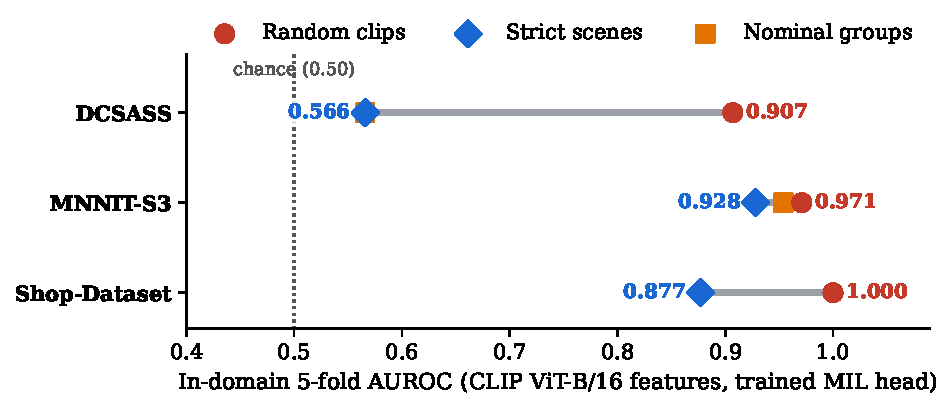
\includegraphics[width=0.92\textwidth]{fig_split_rules.pdf}
\caption{In-domain 5-fold cross-validation AUROC of the same CLIP ViT-B/16 MIL classifier under random clip splits, nominal source groups, and strict scene-disjoint splits. On DCSASS, holding out source folders reduces AUROC from \DCSASSRand{} to \DCSASSStr{} ($-\DCSASSDrop{}$).}\label{fig:split_rules}
\end{figure}

\subsection{Experiment 2: Zero-shot prompts and trained MIL heads show no consistent difference under LODO transfer}

Table~\ref{tab:lodo} and Figs.~\ref{fig:macro_lodo}--\ref{fig:per_dataset_lodo} report leave-one-dataset-out (LODO) performance across all four corpora for the nine zero-shot configurations and the two trained MIL heads. Three findings stand out:

\TableLODO

\begin{enumerate}
    \item \textbf{Zero-shot prompt scoring and supervised LODO training are statistically tied:} Across all nine zero-shot configurations, macro AUROC ranges from 0.644 to \BestZSMacro{}, bracketing the best supervised MIL head on CLIP ViT-B/16 (\BestTRMacro{}; 95\% CI: \BestTRLo{}--\BestTRHi{}). In paired scene-cluster bootstrap comparisons against the CLIP ViT-B/16 trained head (Appendix~\ref{app:paired}, Table~\ref{tab:paired}), paired differences range from $-0.026$ to \TopPairDiff{}, every 95\% confidence interval includes zero (e.g., $[\TopPairLo{}, \TopPairHi{}]$ for \texttt{clip\_b16|zs\_ens8\_mean}), and all nine Holm-Bonferroni adjusted $p$-values equal $1.000$. Thus, supervised weak-label training on three source datasets shows no consistent gain over training-free text-image alignment.

\begin{figure}[ht!]
\centering
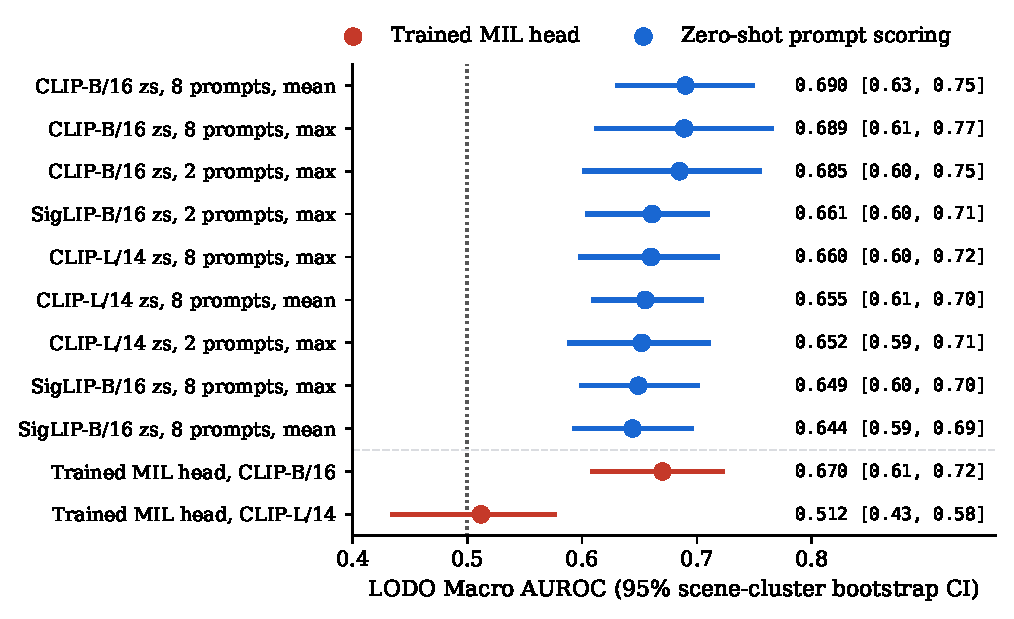
\includegraphics[width=0.95\textwidth]{fig_macro_lodo.pdf}
\caption{Macro AUROC across the four held-out corpora with 95\% scene-cluster bootstrap intervals (500 replicates). The vertical dotted line marks chance performance (0.50).}\label{fig:macro_lodo}
\end{figure}

\begin{figure}[ht!]
\centering
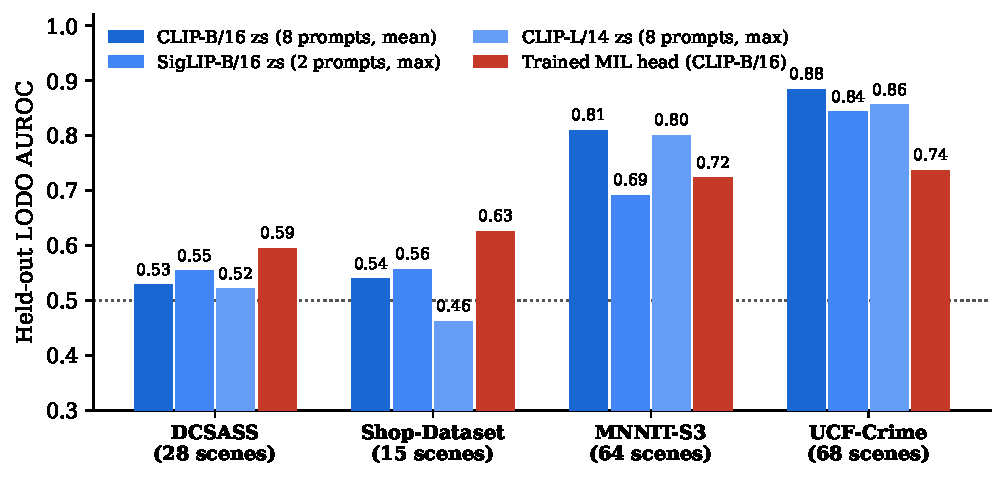
\includegraphics[width=0.95\textwidth]{fig_per_dataset_lodo.pdf}
\caption{Per-dataset LODO AUROC comparison across the four held-out corpora for representative zero-shot prompt configurations and the trained CLIP ViT-B/16 MIL head.}\label{fig:per_dataset_lodo}
\end{figure}

    \item \textbf{Higher-dimensional trained heads overfit severely across domains:} While the trained head on CLIP ViT-B/16 ($D=512$) reaches \BestTRMacro{} macro AUROC, the identical head trained on CLIP ViT-L/14 ($D=768$) scores \LFourteenTRMacro{} macro AUROC and falls below chance on Shop-Dataset (0.328) and UCF-Crime (0.416). Zero-shot CLIP ViT-L/14 outperforming its own trained head by $+0.141$ to $+0.148$ ($p_{\text{Holm}} < 0.001$) reflects cross-domain overfitting in the 768-dimensional supervised head rather than an advantage of larger prompt embeddings.
    \item \textbf{Transferable detection signal is concentrated in two corpora:} UCF-Crime (0.766--0.884 for zero-shot vs.\ 0.737 for the CLIP-B/16 trained head) and MNNIT-S3 (0.650--0.810 for zero-shot vs.\ 0.723--0.798 for trained heads) exhibit consistent above-chance transfer (Fig.~\ref{fig:per_dataset_lodo}). By contrast, DCSASS (0.486--0.611) and Shop-Dataset (0.424--0.645) remain near chance across all evaluated methods once same-store leakage is removed.
\end{enumerate}

\subsection{Experiment 3: Scene regularizers and preprocessing sensitivity}\label{sec:ablations}

Table~\ref{tab:ablations} evaluates whether unsupervised scene-mean centering and Group-DRO improve the trained MIL head (Part A), and how sensitive both paradigms are to minor preprocessing changes (Part B). In Part A, adding Group-DRO to CLIP ViT-B/16 changes LODO macro AUROC from 0.670 to 0.672, while scene-mean centering yields 0.663 (\texttt{center}) and 0.665 (\texttt{center+dro}); on CLIP ViT-L/14, \texttt{center} ($0.541$), \texttt{dro} ($0.522$), and \texttt{center+dro} ($0.549$) partially mitigate cross-domain overfitting ($0.512 \to 0.549$) but remains well below zero-shot CLIP ViT-L/14 ($0.652$--$0.660$).

\TableAblations

Part B of Table~\ref{tab:ablations} compares our canonical preprocessing pipeline (OpenAI CLIP green-channel mean $0.4578275$ and \texttt{ffmpeg} timestamp seeking for videos $>20$\,s) against a perturbed run that used a slightly shifted green-channel mean ($0.4728275$) and a file-size seek rule ($>15$\,MB). Training-free zero-shot prompt scoring is nearly invariant to this perturbation ($\Delta = +0.002$ on CLIP-B/16 \texttt{zs\_ens8\_mean}, $0.690 \to 0.692$), whereas the supervised CLIP-B/16 MIL head drops by $-0.055$ macro AUROC ($0.670 \to 0.615$) and strict-scene 5-fold CV drops by $-0.038$ on DCSASS ($0.566 \to 0.528$) and $-0.069$ on Shop-Dataset ($0.877 \to 0.808$). This contrast highlights the fragility of supervised heads fitted to small surveillance corpora: minor shifts in feature normalization and frame decoding alter the learned decision boundary enough to turn a statistical tie ($+0.020$, CI: $[-0.051, +0.085]$) into an apparent gap ($+0.077$).

\section{Discussion, Limitations, and Ethical Considerations}\label{sec:discussion}

\subsection{Why do in-domain and cross-dataset rankings diverge?}

Our experiments resolve an apparent contradiction in the retail anomaly detection literature: studies evaluated on random splits of DCSASS or Shop-Dataset report AUROC above 0.90, yet models deployed on unseen cameras struggle. On DCSASS, each of the 28 source recordings was sliced into 32 short clips; random clip partitioning guarantees that approximately 25 clips from the exact same camera view and lighting condition appear in the training set for every 7 test clips. A 2-layer MLP on frozen CLIP embeddings exploits this shared scene appearance to achieve \DCSASSRand{} AUROC, but drops to \DCSASSStr{} when evaluated on held-out incident folders and 0.595 under LODO transfer. Conversely, on MNNIT-S3, where theft actions are visually prominent, the trained head achieves \MNNITStr{} under strict in-domain scene splits and 0.723--0.798 under LODO transfer, while 8-prompt zero-shot ensembles reach 0.749--0.810 without seeing a single training video from any shoplifting dataset.

\subsection{Limitations}

Three technical limitations bound the scope of our conclusions:
\begin{enumerate}
    \item \textbf{Frozen frame-level features without fine-grained motion modeling:} We evaluate frozen CLIP and SigLIP frame representations sampled at $T=32$ frames per clip. Subtle hand-to-pocket concealments occurring over sub-second intervals or requiring high-resolution bounding-box or human-pose tracking may not be captured at $224 \times 224$ full-frame resolution.
    \item \textbf{Video-level rather than frame-level evaluation:} Because public copies of MNNIT-S3 and Shop-Dataset provide only clip-level binary labels rather than frame-level temporal annotations, our benchmark evaluates clip-level anomaly ranking rather than temporal localization IoU.
    \item \textbf{Unsupervised scene clustering in datasets lacking camera metadata:} While DCSASS provides exact incident folder labels, camera IDs are absent in MNNIT-S3, Shop-Dataset, and UCF-Crime. Our spherical $k$-means scene clusters provide a reproducible visual proxy for camera groupings, but releasing future benchmarks with ground-truth camera and store identifiers remains essential.
\end{enumerate}

\subsection{Ethical and deployment considerations}

Automated shoplifting detection systems carry significant risks of false accusations and disproportionate scrutiny if deployed without human oversight. At the macro AUROC levels observed under strict scene-disjoint and cross-dataset evaluation (0.644--\BestZSMacro{}), neither supervised MIL heads nor zero-shot vision-language models are reliable enough for autonomous retail alerting or law-enforcement action. Any practical deployment must treat anomaly scores strictly as assistive triage signals reviewed by trained personnel, audit false-alarm rates across camera viewpoints and demographics, and avoid retaining biometric identifiers.

\section{Conclusion and Methodological Recommendations}\label{sec:conclusion}

Based on our audit of \TotalClips{} clips across four public shoplifting corpora, we show that random sub-clip splits inflate in-domain AUROC by up to \DCSASSDrop{}, and that under leave-one-dataset-out transfer there is no consistent difference between training-free zero-shot prompt scoring ($0.644$--\BestZSMacro{} macro AUROC) and supervised MIL heads (\BestTRMacro{} on CLIP ViT-B/16). We recommend four reporting standards for future retail anomaly detection research:
\begin{enumerate}
    \item \textbf{Abolish random sub-clip splits:} Always partition by source recording, physical camera ID, or visual scene cluster, and report leave-one-dataset-out (LODO) transfer across multiple corpora.
    \item \textbf{Report per-dataset and unweighted macro metrics:} Never pool predictions across datasets with different positive base rates into a single ROC curve, as dataset-identity priors alone yield \PooledAUROCID{} pooled AUROC at \MacroAUROCID{} macro AUROC.
    \item \textbf{Include a training-free zero-shot prompt baseline:} Any proposed supervised architecture using vision-language features should be compared against training-free cosine similarity with fixed prompts on the exact same frozen features.
    \item \textbf{Report scene-cluster bootstrap intervals and multiple-comparison adjustments:} Because scenes---not sub-clips---are the independent sampling units in surveillance benchmarks, uncertainty should be quantified by resampling scenes with replacement and adjusting for multiple comparisons.
\end{enumerate}

\backmatter

\bmhead{Data and code availability}
The benchmark pipeline, self-contained execution notebook, configuration files, and pre-computed evaluation tables are publicly available at \url{https://github.com/NaveenKumarGottipalli/Shopliftingdetector}, with the curated multi-corpus dataset index hosted at \url{https://huggingface.co/datasets/NaveenKumarGottipalli/Shoplifting_DataCollection}.

\bmhead{Competing interests}
The author declares no competing financial or non-financial interests.

\bmhead{Funding}
No external funding was received for conducting this study.

\appendix

\section{Paired Bootstrap Comparisons and Multiple-Testing Adjustment}\label{app:paired}

Table~\ref{tab:paired} reports the paired differences in LODO macro AUROC ($\Delta = \text{AUROC}_{\text{zero-shot}} - \text{AUROC}_{\text{trained}}$) across all 500 scene-cluster bootstrap replicates, along with two-sided bootstrap $p$-values ($p_{\text{raw}}$), step-down Holm-Bonferroni adjusted $p$-values ($p_{\text{Holm}}$), and the number of datasets (out of 4) on which the zero-shot method achieves a higher point-estimate AUROC.

\TablePaired

\bibliography{refs}

\end{document}
